\section{Introduction}

Mental health has been a significant challenge in global healthcare. Nearly 1 in 5 U.S. adults live 
with a mental illness or condition~\citep{NIMHMental}, and there are about 1 billion people suffering from mental disorders worldwide~\citep{UNMental}. Due to the stigma of mental disorders and lack of professional mental health services, many people cannot receive proper diagnose or treatment for their conditions. Social Media can be a promising source for studies on this problem, as we may detect hidden traces of mental disorders from the symptoms that users may reveal in their free sharing, and provide pertinent help for those in need. Consequently, Mental Disease Detection (MDD) from social media has received increasing attention \citep{coppersmith2015adhd,cohan2018smhd}. 

\begin{figure}[t]
    \centering
    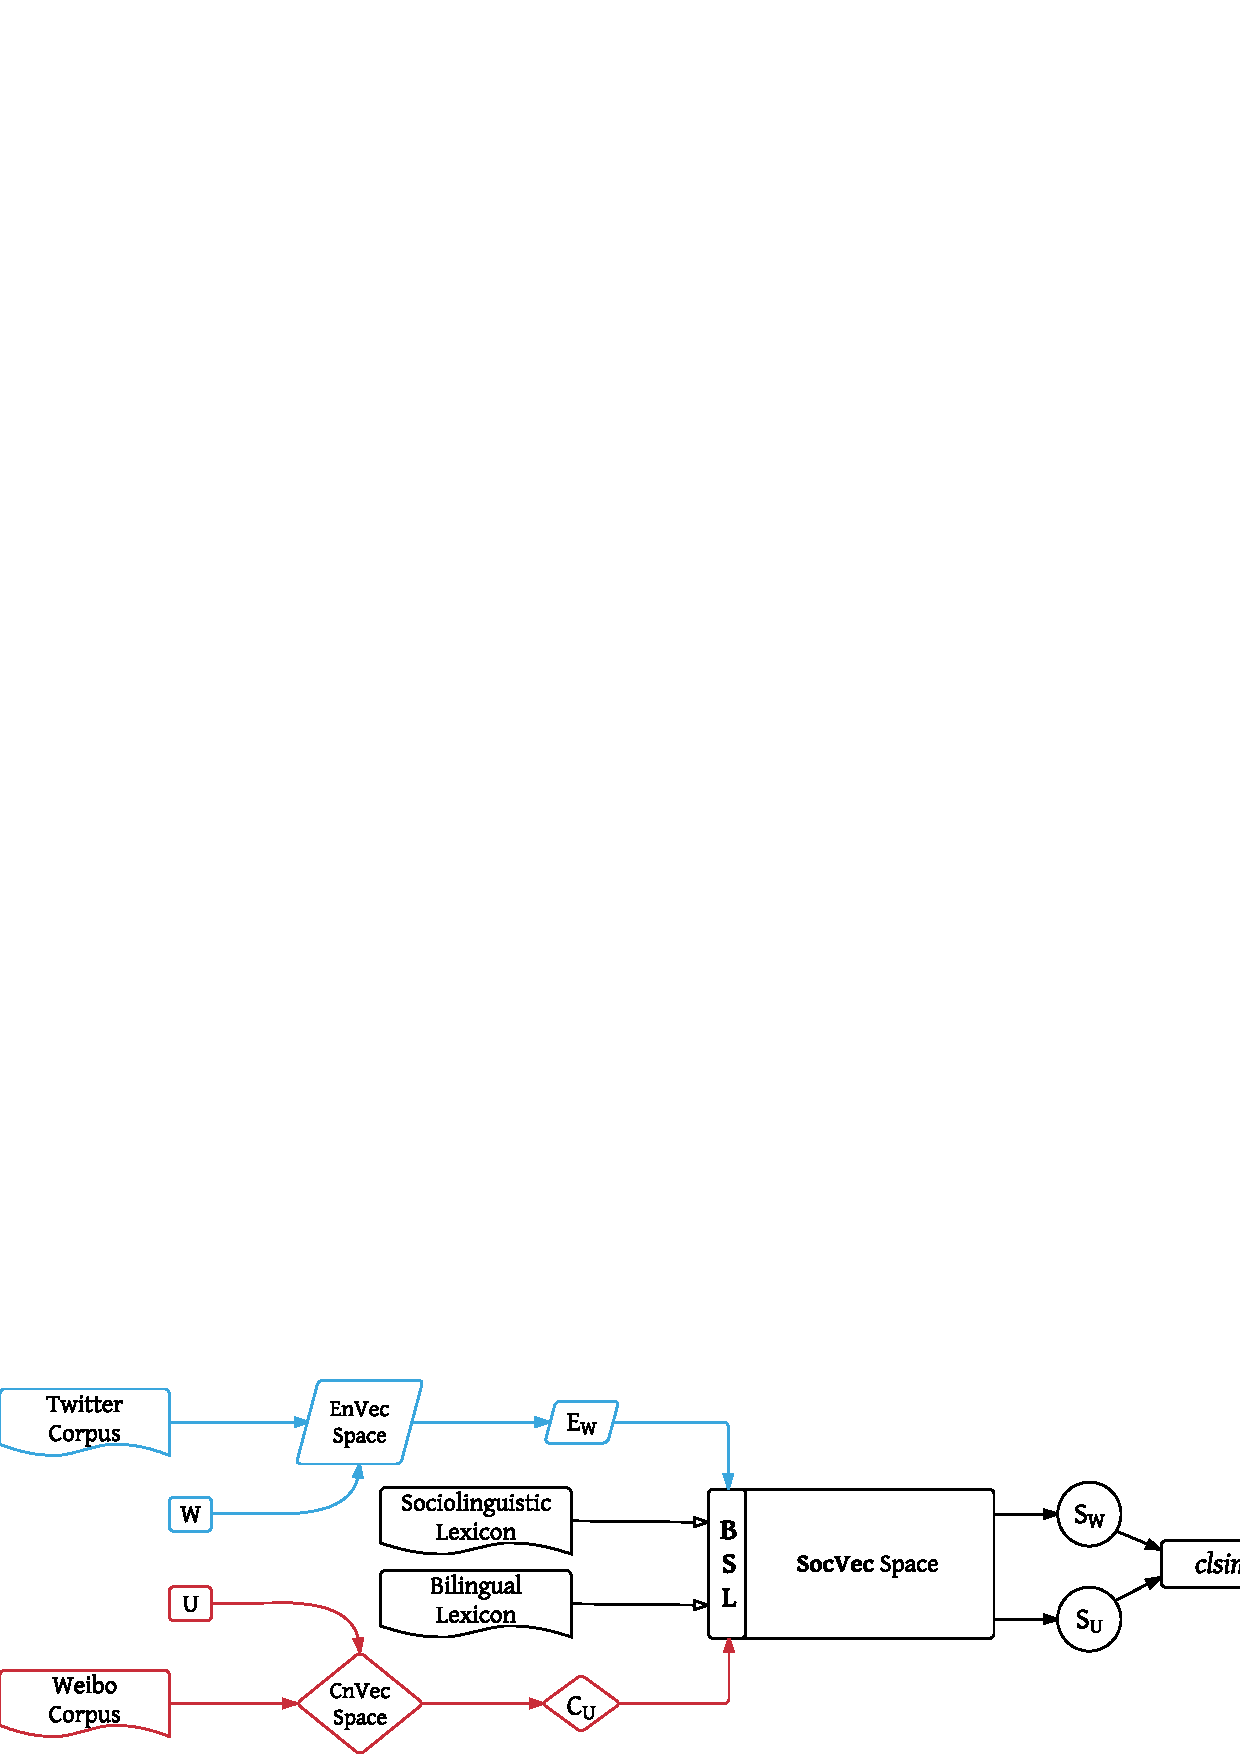
\includegraphics[width=1.0\columnwidth]{figures/overview.pdf}
    \caption{Comparison between text-based and the proposed symptom-assisted 
mental disease detection method, which leverages psychiatric knowledge for 
symptom identification to improve the effectiveness and interpretability of MDD.}
    \label{fig:overview}
\end{figure}

However, most automatic MDD methods still struggle in this task, especially for their unsatisfying generalizability and explainability. Firstly, these models may learn dataset-specific spurious correlations between certain words and the labels (usually diseases), and thus fail to generalize~\citep{harrigian2020models}. Moreover, most deep learning based methods work as black boxes, and cannot provide explanations for their prediction, which differs from the clinical practice which leverages symptom-based diagnostic criterions from authoritative manuals like DSM-5 \citep{american2013diagnostic}. Therefore, it may be hard for current MDD methods to gain trust from their users. 
%myw 最后一句有点武断; 前一句还是明确是symptom-based *disease* diagnosis 把你的symptom重要性体现
%zhiling symptom的重要性在下一段中集中论述

To tackle these issues, there has been a rising interest in utilizing \textit{symptoms} for MDD, as they are the bases that human psychiatrists use to make diagnoses. Pioneering research has shown their potential benefits of improving the accuracy, generalizability and interpretability of MDD \citep{lee2021micromodels,nguyen2022improving,zhang22risky}. Nevertheless, due to the lack of large-scale annotated corpus for supervised learning, they can only extract symptom features with unsupervised/weakly supervised methods or simple pattern matching, which may not guarantee the quality of the extracted features. Moreover, most of these works only focus on the detection of depression. However, many mental disorders may share similar set of symptoms. For example, depressed mood can not only be seen on the patient of depression, but also those suffering from bipolar disorder, anxiety, etc. Jointly modeling the symptoms of multiple diseases may enhance the performance on all classes. 

These limitations call for the establishment of a large-scale, multi-disease annotated dataset for symptom identification, which will face many novel challenges. Initially, the symptoms of multiple diseases are scattered over the different chapters of DSM-5 and other materials. Similar symptoms would have varied expressions in different places, which causes difficulty in setting up the annotation standard. Furthermore, the free and diverse language style on social media \citep{yadav2020identifying} can make the retrieval of candidate posts for annotation difficult. Last but not least, the relatively large amount of symptoms from different disorders and the nuanced differences and similarities between them make it hard to get high-quality annotations (i.e. inter-rater agreement will be low).  

%myw 以下,最好描述下novel data annotation framework that involves uncertainty into labelling process
%zhiling 出于空间的考虑,在目前的8页版本里面就暂时不加了,对于突出这篇文章的主要贡献来说应该足够了
In this work, we propose a novel data annotation framework, and introduce the first multi-disease symptom identification dataset based on social media posts, \textit{PsySym} (\textbf{Psy}chiatric-disorder \textbf{Sym}ptoms), which contains the multi-label annotations of 38 symptom classes from 7 mental diseases on 8,554 Reddit post sentences. We establish our annotation target (symptom classes) mainly based on the diagnostic criterions from DSM-5, with symptom descriptions on clinical questionnaires as supplementary. We leverage embedding-based retrieval methods \citep{reimers-2019-sentence-bert} instead of keyword matching to get the candidate sentences for annotation, which can effectively constrain our efforts to a precise but diverse subset of posts for efficient annotation. To guarantee the quality of data, we apply several quality control approaches, and divide the annotation tasks by separate diseases so as to reduce the cognitive burdens of annotators, resulting in high inter-rater agreement.

Finally, we propose a symptom-assisted MDD framework (Figure \ref{fig:overview}). We use models trained on PsySym to extract symptom features for MDD, outperforming strong BERT-based baseline \citep{devlin2018bert}. We also explore the interpretability of symptom identification for MDD. We find that they can reasonably provide DSM-5 compliant explanations for diagnosed patients. We will also show that symptom-based interpretations can also help us find incorrect labels in automatically constructed MDD datasets, indicating their further potential. 

Our contributions are:
\begin{itemize}
    \item We build the first social-media based symptom identification dataset of multiple mental diseases, \textit{PsySym}, with novel annotation framework to guarantee the diversity and quality of the dataset.
    \item We propose symptom-assisted MDD, which leverages the features extracted from PsySym-trained models, and can outperform strong baselines in MDD.
    \item We demonstrate the intuitive interpretability for MDD results enabled by symptoms, and its promising applications with case studies. 
\end{itemize}
